% НИР
\documentclass[master, och, times, nir]{sty/SCWorks}

\usepackage[T2A]{fontenc}
\usepackage[utf8]{inputenc}
\usepackage{graphicx}
\usepackage{float}

\usepackage[sort,compress]{cite}
\usepackage{amsmath}
\usepackage{amssymb}
\usepackage{amsthm}
\usepackage{longtable}
\usepackage{array}
\usepackage[english,russian]{babel}
\usepackage{amsfonts}
\usepackage{commath}
\usepackage{amsthm}

\usepackage[colorlinks=true]{hyperref}

\usepackage{listings}

\usepackage[ruled,vlined,linesnumbered,resetcount,algosection]{algorithm2e}

\usepackage{algpseudocode}

\usepackage{longtable,rotating}
\usepackage{threeparttable}

% для кода
\usepackage{fancyvrb}
\DefineShortVerb{\|}

% для картинок
\usepackage{chngcntr}
\counterwithin{figure}{section}

\theoremstyle{plain}
\newtheorem{thethm}{Теорема}[section]
\newtheorem{lemma}{Лемма}[section]
\newtheorem{note}{Замечание}[section]
\newtheorem{proposition}{Предложение}[section]
\newtheorem{exmp}{Пример}[section]
\newtheorem{problem}{Проблема}[section]

\theoremstyle{definition}
\newtheorem{defn}{Определение}[section]

\numberwithin{equation}{section}

\SetKwInput{KwData}{Исходные параметры}
\SetKwInput{KwResult}{Результат}
\SetKwInput{KwIn}{Входные данные}
\SetKwInput{KwOut}{Выходные данные}
\SetKwIF{If}{ElseIf}{Else}{если}{тогда}{иначе если}{иначе}{конец условия}
\SetKwFor{While}{до тех пор, пока}{выполнять}{конец цикла}
\SetKw{KwTo}{от}
\SetKw{KwRet}{возвратить}
\SetKw{Return}{возвратить}
\SetKwBlock{Begin}{начало блока}{конец блока}
\SetKwSwitch{Switch}{Case}{Other}{Проверить значение}{и выполнить}{вариант}{в противном случае}{конец варианта}{конец проверки значений}
\SetKwFor{For}{цикл}{выполнять}{конец цикла}
\SetKwFor{ForEach}{для каждого}{выполнять}{конец цикла}
\SetKwRepeat{Repeat}{повторять}{до тех пор, пока}
\SetAlgorithmName{Алгоритм}{алгоритм}{Список алгоритмов}

\algrenewcommand\algorithmicfunction{\textbf{Функция}}
\algrenewcommand\algorithmicprocedure{\textbf{Процедура}}
\algrenewtext{EndFunction}{\textbf{Конец функции}}
\algrenewtext{EndProcedure}{\textbf{Конец процедуры}}


\begin{document}



% Кафедра (в родительном падеже)
\chair{дискретной математики}
% Тема работы
\title{}
% Курс
\course{2}
% Группа
\group{271}
% Специальность/направление код - наименование
\napravlenie{09.04.01 "--- Информатика и вычислительная техника}

\term{4}

% Фамилия, имя, отчество в родительном падеже
\author{Шарова Александра Вадимовича}
% Заведующий кафедрой
\chtitle{к.\,ф.-м.\,н., доцент} % степень, звание
\chname{Л.\,Б.\,Тяпаев}
%Научный руководитель (для реферата преподаватель проверяющий работу)
\satitle{к.\,ф.-м.\,н., доцент} %должность, степень, звание
\saname{Л.\,Б.\,Тяпаев}
% Руководитель практики от организации (только для практики,
% для остальных типов работ не используется)
\patitle{к.\,ф.-м.\,н., доцент}
\paname{Д.\,Ю.\,Петров}

% Год выполнения отчета
\date{2020}

\maketitle
\tableofcontents


\intro

Цель данной научно-исследовательской работы -- разработка многопоточного варианта библиотеки для работы с $p$-адической арифметикой.

В течение семестра была доработана однопоточная библиотека для работы с $p$-адической арифметикой, а затем расширена с помощью применения параллельного программирования на многопоточный случай. Как для многопоточной, так и для однопоточной библиотеки были произведены тесты производительности, где в качестве примера использовались такие прикладные задачи как нахождение решения СЛАУ, ОДУ, вычисление собственных чисел и собственных значений векторов матрицы, вычисление матричной экспоненты. Все тесты производились с использованием чисел из таких числовых полей, как $\mathbb{Q}_2$, $\mathbb{Q}_3$, $\mathbb{Q}_5, \mathbb{Q}_5$ и $\mathbb{Q}_{23}$.

В апреле на студенческой научной конференции был представлен доклад о возможностях использования $p$-адической арифметики в ЭВМ, где были рассмотрены в том числе и вопросы производительности на примере задачи вычисления матричной экспоненты.

\section{Разработка многопоточной библиотеки для работы с $p$-адической арифметикой}

\subsection{Описание многопоточной $p$-адической арифметики}

Многопоточный алгоритм для $p$-адических чисел впервые был предложен Моррисоном \cite{bib:numbers:morrison}. Алгоритм основан на китайской теореме об остатках, которая расширена на случай использования рациональных чисел. Процесс декодирования $p$-адической последовательности в этом случае выглядит следующим образом: если $r \sim \{r_1,r_2,\cdots, r_s\}$ является представлением остатка рационального числа $a$ по модулям $\{r_1,r_2,\cdots, r_s\}$, где наибольший общий делитель $GCD(p_i, p_j) =1 \; \forall i \neq j$, то тогда процесс декодирования осуществляется с помощью алгоритма \ref{algo:decoding}\cite{bib:numbers:newman}\cite{bib:numbers:dixon}.


\begin{algorithm}
\DontPrintSemicolon % Some LaTeX compilers require you to use \dontprintsemicolon instead
\Begin {
	$p$ := $\prod\limits_{i=1}^{s} p_i $ \\
	\For{$i \gets 1$ \textbf{to} $s$} {
		найти $p_{i}^{'}: \frac{p}{p_i}p_{i}^{'} \equiv 1 \pmod {p_i}$
	}
	$\overline{r}=\sum\limits_{i=1}^{s} p_{i}^{'}r_i \pmod p$


	$u_{-1}=p, u_0=\overline{r}$ \\
	$v_{-1}=0, v_0=1$ \\
	$i=-1$ \\
	\While{$u_i \textless \sqrt{p}$} {
		$q_i=\lfloor{\frac{u_{i-1}}{u_i}}\rfloor$ \\
		$u_{i+1}=u_{i-1}-q_i u_i$ \\
		$v_{i+1}=v_{i-1}+q_i v_i$ \\
		$i = i +1$
	}


	\Return $r=((-1)^{i} \frac{u_i}{v_i})$
}
\caption{декодирование $p$-адического числа.}
\label{algo:decoding}
\end{algorithm}

При комбинации $p$-адической арифметики и китайской теоремы об остатках получается многопоточный алгоритм для $p$-адической арифметики, представленный в виде блок-схемы на рисунке \ref{img:multi:schema}.

\begin{figure}[H]
\centerline{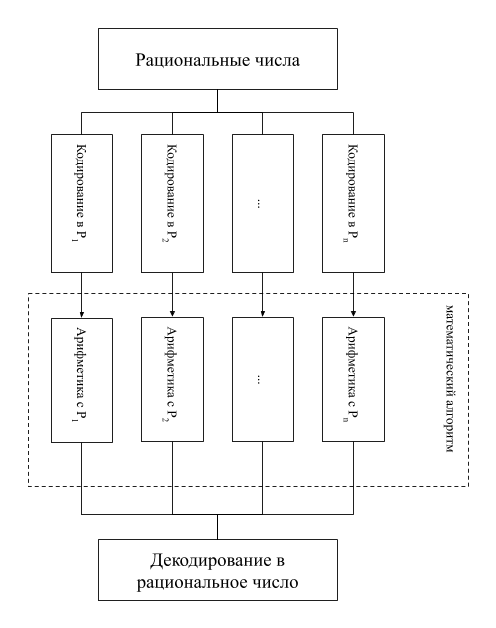
\includegraphics[width=0.7\linewidth]{images/multi/schema.png}}
\caption{Китайская теорема об остатках, скомбинированная с $p$-адической арифметикой.}
\label{img:multi:schema}
\end{figure}

Далее рассмотрим метод для определения наличия или отсутствия переполнения. Для начала необходимо ввести определение переполнения.

\begin{defn}
Рациональное число $\frac{a}{b} \pmod{p_i}$, которое определяет последовательность $r \sim \{r_1,\cdots, r_s\}$ при условии, что $\gcd{(a, b)}=1$, не может быть однозначно восстановлено с помощью обратного преобразования \ref{th:backward_mapping} для  алгоритмов, которые основаны на китайской теореме об остатках, примененной для простых чисел $\{p_1,\cdots, p_s\}$. Данная ситуация называется переполнением.
\end{defn}

Один из методов для обнаружения переполнения -- это предсказывание верхней границы вычислений, а затем определение размера простого множества $\{p_1,p_2, \cdots, p_n\}$, как это сделано в \cite{bib:numbers:matula}. Другой способ для определения переполнения - использование дополнительных цифр в последовательности $p$-адического числа, как это сделано в \cite{bib:numbers:hensel:overflow}. Этот метод может определять переполнение на основе набора простых чисел $\{p_1,\cdots, p_n\}$ и вычисления остаточного набора чисел. В этом методе каждая числовая последовательность должна иметь дополнительные числа, используемые для сохранения последовательности, состоящей из $k$ чисел.
С помощью набора простых чисел $\{p_1,p_2, \cdots, p_i, p_{i+1}, \cdots, p_{i+k}\}$ для любого рационального числа $x$ получается последовательность $\{r_1 = x \pmod{p_1},\cdots, r_{i+k}= x\pmod{p_{i+k}}\}$, запишем ее как $x \sim \{r_1, r_2, \cdots, r_{i}, r_{i+1}, \cdots, r_{i+k}\}$.
Во время процесса определения наличия переполнения это будет рассматриваться как

\begin{equation}
x \sim (r_0, r_1, \cdots, r_i, r_{i+1}, \cdots, r_{i+k}),
\end{equation}

\noindent где $ r_{i+1}, \cdots, r_{i+k}$ является проверочной частью последовательности.

Теперь можно ввести критерий существования или отсутствия переполнения, который используется в программной реализации $p$-адической арифметики.

\begin{defn}
Переполнение для последовательности $x$ случится, если

\begin{equation}
Decoding(x,i) \neq Decoding(x,i+k),
\end{equation}

\noindent и не случится, если

\begin{equation}
Decoding(x,i) = Decoding(x,i+k).
\end{equation}
\end{defn}

\subsection{Многопоточный метод решения СЛАУ}
Стандартная схема вычисления вектора решения $\boldsymbol{x}$ для СЛАУ $\boldsymbol{A}\cdot \boldsymbol{x} = b$ содержит представление рациональных чисел с помощью $p$-адических чисел в виде кода Гензеля и выполнении операций над данными числами. Однако, как видно из теоремы \ref{th:backward_mapping}, представление чисел в виде кода Гензеля возможно только когда, ожидаемый результат будет принадлежать множеству $\mathbb{F}_{p,r}$. Это значит, что необходимо  произвести правильный выбор чисел $p$ и $r$.


Перед тем как переходить к описанию параллельного метода решения СЛАУ, необходимо представить последовательный метод Гаусса.

\begin{problem}
Пусть дана матрица $\boldsymbol{A} \in \mathbb{Q}^{n \times n}$ и вектор $\boldsymbol{b} \in \mathbb{Q}^{n}$. Необходимо найти вектор $\boldsymbol{x}=(x_1,\cdots,x_n) \in \mathbb{Q}^{n}$ при котором

\begin{equation}
\boldsymbol{A}\cdot \boldsymbol{x} = b.
\end{equation}

\end{problem}

Для начала предположим, что $\boldsymbol{A} \in \mathbb{Z}^{n \times n}$ и $\boldsymbol{b} \in \mathbb{Z}^{n}$. Согласно правилу Крамера

\begin{equation}\label{formula:kramer}
x_i=\frac{\Delta_i}{\Delta},
\end{equation}

\noindent где $\Delta$ -- это определитель матрицы $A$, а $\Delta_i$ -- это определитель, получаемый из определителя $\Delta$ путем замены $i$-го столбца на столбец свободных членов. Известно, что если взять для любой матрицы $\mathbb{Z}^{n \times n}$ число $a$, которое будет максимальным среди остальных элементов, то оно будет удовлетворять неравенству

\begin{equation}
\mid M \mid \leq n!a^n.
\end{equation}

\noindent Из этого выражения и формулы \ref{formula:kramer} получаем, что числитель и знаменатель для любого $x_i$ ограничен числом $n!a^n$, где $a$ -- максимальное значение матрицы $A$. Из этого ограничения можно определить число $r \in \mathbb{F}_{p,r}$ для данного простого числа $p$. Из определения следует, что

\begin{equation}\label{formula:det:1}
n!a^b \leq \sqrt{\frac{p^r-1}{2}}.
\end{equation}

Принимая во внимание квадрат в левой стороне неравенства, получаем, что

\begin{equation}
2{(n!a^n)}^2+1\leq p^r.
\end{equation}

\noindent Неравенство в свою очередь аналогично следующему:

\begin{equation} \label{eq:matrix:r}
r \geq log_p(2{(n!a^n)}^2+1).
\end{equation}

Известно, что неравенство Адамара, рассмотренное, в например, \cite{bib:numbers:mignotte} и \cite{bib:numbers:marcus}, представляет следующее ограничение для определителя:

\begin{equation}
{\mid A \mid}^2 \leq \prod\limits_{i=1}^{n}{\bigg(\sum\limits_{j=1}^{n} a^2_{i,j} \bigg)}^{\frac{1}{2}}
\end{equation}

\noindent Из этого неравенства и неравенства \ref{formula:det:1} следует условие:

\begin{equation}
p^r \leq \sum\limits_{i=1}^{n} {\mid b_i \mid} \prod\limits_{i=1}^{n}{\bigg(\sum\limits_{j=1}^{n} a^2_{i,j} \bigg)}^{\frac{1}{2}}.
\end{equation}

Должно быть отмечено, что оба ограничения являются строгими и меньший выбор чисел $p$ и $r$ частно достаточен. В обычном случае $A \in \mathbb{Q}^{n \times n}$ и и $\boldsymbol{b} \in \mathbb{Q}^{n}$ ограничением для числителя и знаменателя для числа $x_i$ становится $n!a^{n(n+1)}$.

\begin{thethm}
Пусть $n_1,n_2,\dots, n_k$ -- натуральные попарно взаимно простые числа, а $r_1,r_2,\dots,r_k$ -- некоторые целые числа, тогда существует такое целое число $M$, которое будет решением системы сравнений:

\begin{equation}
\begin{cases}
M \equiv r_1 \pmod {n_1}, \\
M \equiv r_2 \pmod {n_2}, \\
\dots \\
M \equiv r_k \pmod {n_k}.
\end{cases}
\end{equation}

\noindent При этом для любых двух решений $A$ и $B$ этой системы справедливо

\begin{equation}
A \equiv B \pmod {n_1,n_2,\dots,n_k},
\end{equation}

\noindent то есть решение системы сравнений существует и единственно по модулю $n_1,n_2,\dots,n_k$.
\end{thethm}


Будем описывать параллельный алгоритм решения СЛАУ для $k$ процессов (или независимых потоков). Для начала нужно вычислить $k$ простых чисел $p_1, \dots, p_k$ случайным образом, которые удовлетворяют длине кода $r$ так, что числа из вектора $x$ содержатся в $\mathbb{F}_{g,r}$, где $g=p_1,\dots,p_k$.
Запустим $k$ параллельных задач. Каждая из них вычисляет образ в отношении одного простого числа в представлении рациональных элементов, то есть $H_{p_i,r}(A)$ и $H_{p_i,r}(b)$.
Затем каждый процесс запускает метод Гаусса.

\newpage

\begin{algorithm}
\DontPrintSemicolon % Some LaTeX compilers require you to use \dontprintsemicolon instead

\KwIn{ $n$: степень системы \newline
       $A=(a_{i,j}) \in \mathbb{Q}^{n \times n}$: квадратная, $\dim(A)=n \times n$ \newline
       $b=(a_{1,n+1},\dots,a_{n,n+1}) \in \mathbb{Q}^{n}$: $\dim(b)=n$ \newline
       $p$: простое число }

\KwOut{$x=(x_1,\dots,x_n) \in \mathbb{Q}^{n}$: решение $Ax = b$ если существует.}

\Begin {
Найти максимум $a$ среди числителей и знаменателей среди чисел входящих в состав $A$ и $b$.

Вычислить порядок числа $r$ по формуле \ref{eq:matrix:r}.

Преобразовать числа входящие из $A$ и $b$ в код Гензеля $H_{p,r}$.

l := 0\;
\For{$i \gets 1$ \textbf{to} $n$} {
  l := l + 1 \;
  \For{$j \gets 1$ \textbf{to} $n+1$} {
      Поделить $a_{i,j}$ на $a_{i,i}$.
  }
   \For{$h \gets l+1$ \textbf{to} $n$} {
      Умножить $i$-ю строку на $a_{h,l}$\;
      Вычесть полученную $i$-ю строку на $h$-ю строку системы полученную последней операцией. Это новая $h$-я строка.
  }
}

Восстановить $H_{p,r}(x_1), \cdots, H_{p,r}(x_n)$ из полученной треугольной матрицы.
}


\caption{Алгоритм Гаусса для $p$-адической арифметики.}
\label{algo:gauss}
\end{algorithm}


Представленный алгоритм \ref{algo:gauss} вычисляет решения $x^{(i)} \in \mathbb{H}_{p_i,r}^n$ для $i = \overline{1,k}$. После получения всех $x^{(i)}$ выполняется $k$ параллельных запусков алгоритма расширенной китайской теоремы об остатках. Будем применять параллельную версию расширенного алгоритма китайской теоремы об остатках описанную в \cite{bib:numbers:limongelli} для каждой последовательности компонентов $x_j^{(1)}, \dots, x_j^{(k)}$, получая компоненты $x_j \in \mathbb{H}_{p_1,\dots,p_k,r}$ вектора решения $x$.
Из предположений, сделанных для числа $r$, полученный список результатов $\{x^{(1)},\dots,x^{(k)}\}$ может быть преобразован обратно в вектор $x \in \mathbb{F}_{g,r}^n$ с помощью китайской теоремы об остатках. Из теоремы \ref{th:hensel} известно, что если решение существует в $\mathbb{F}_{g,r}$, то оно уникально.
После этого результат $x$ должен быть сконцентрирован из $p$-адического представления в обычное с помощью теоремы \ref{th:backward_mapping}, примененной параллельно к каждому из компонентов. Схема параллельных вычислений представлена ниже на рисунке \ref{img:multi:gauss}.

\begin{figure}[H]
\centerline{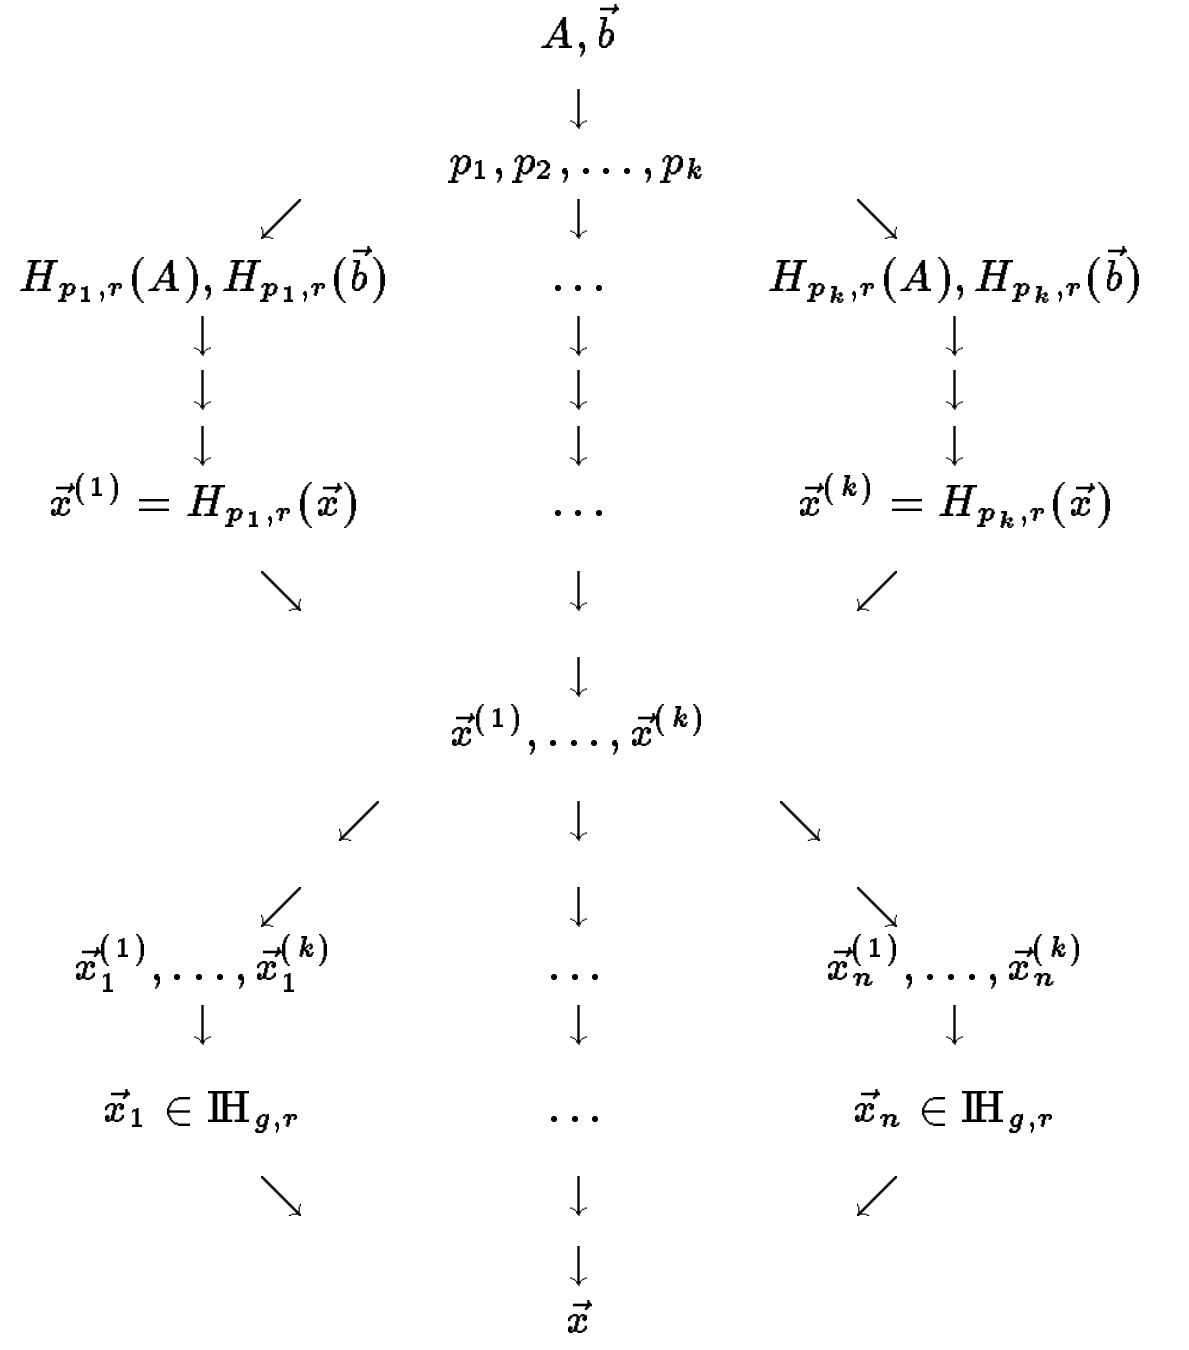
\includegraphics[width=0.7\linewidth]{images/multi/native.png}}
\caption{Схема параллельного алгоритма для нахождения решения СЛАУ методом Гаусса.}
\label{img:multi:gauss}
\end{figure}


В случае с матрицами очень больших размерностей, в разы больших, чем количество доступных процессоров, могут быть использованы стандартные методы для распараллеливания матричных операций.


\subsection{Многопоточный метод для вычисления собственных значений и собственных векторов}

Нахождение собственных значений и собственных векторов матриц - одна тех сложных вычислительных задач, с которой часто приходится сталкиваться специалисту, занимающемуся проектированием или анализом больших технических систем.  В электрических и механических системах собственные числа отвечают собственным частотам колебаний, а собственные векторы характеризуют соответствующие формы колебаний. В теории динамических систем и связанных с ними системах линейных дифференциальных уравнений знание собственных значений позволяет определить характер поведения системы во времени и решить вопрос об устойчивости такой системы. Оценка величин критических нагрузок при расчете строительных конструкций также основана на информации о собственных значениях и собственных векторах матриц.

Одним из методов нахождения собственных векторов и собственных значений является метод Якоби, или метод вращений. Метод Якоби был предложен Карлом Густавом Якоби в 1846 году и представляет собой итерационный алгоритм вычисления собственных значений и собственных векторов симметричной матрицы. Метод основан на построении последовательности матриц, которые ортогонально подобны исходной матрице и имеют монотонно убывающие до нуля суммы всех внедиагональных элементов. Данный метод без существенных изменений переносится на эрмитовы и косоэрмитовы матрицы. В данной работе будем рассматривать только метод, где матрица $A$ является вещественной и симметричной. Алгоритмы для случая комплексной эрмитовой матрицы можно посмотреть в \cite{bib:numbers:voevodin}.

Прежде чем переходить к описанию алгоритма и рассмотрению его особенностей, связанных с применением $p$-адической арифметики, необходимо ввести несколько определений.


\begin{defn}
Число $\lambda$ называется собственным значением матрицы $A$, если существует такой ненулевой вектор $x=(x_1,x_2,\cdots,x_n)$, удовлетворяющий уравнению

\begin{equation}
Ax=\lambda x
\end{equation}

\noindent и называемый собственным вектором матрицы $A$, отвечающий собственному значению $\lambda$.
\end{defn}


\begin{defn}
Матрицей вращения или матрицей поворота называется ортогональная матрица, которая используется для выполнения собственного ортогонального преобразования в евклидовом пространстве. При умножении любого вектора на матрицу поворота длина вектора сохраняется. Определитель матрицы поворота равен единице.
\end{defn}

Будем описывать параллельный алгоритм для нахождения собственных значений и собственных векторов матрицы $A$ для $k$ процессов (или независимых потоков). Для начала случайным образом нужно вычислить $k$ простых чисел $p_1, \dots, p_k$, которые удовлетворяют длине кода $r$ так, что числа из вектора $x$ содержатся в $\mathbb{F}_{g,r}$, где $g=p_1,\dots,p_k$.
Запустим $k$ параллельных задач. Каждая из них вычисляет образ в отношении одного простого числа в представлении рациональных элементов, то есть $H_{p_i,r}(A)$ и $H_{p_i,r}(b)$. После этого выполняется последовательный алгоритм Якоби.

Алгоритм \ref{algo:jacoby} вычисляет значения $\lambda_i$ и $x_i$ для матрцы $A$. После получения всех собственных векторов и всех собственных чисел выполняется $k$ параллельных запусков китайской теоремы об остатках. Будем применять параллельную версию китайской теоремы об остатках, описанную в \cite{bib:numbers:limongelli} для каждой последовательности компонентов $x_j^{(1)}, \dots, x_j^{(k)}$ и $\lambda_j^{(1)}, \dots, \lambda_j^{(k)}$, получая компоненты $x_j \in \mathbb{H}_{p_1,\dots,p_k,r}$ и $\lambda_j \in \mathbb{H}_{p_1,\dots,p_k,r}$. Вспомогательные функции |maxind|, |rotate| и |update| для алгоритма \ref{algo:jacoby} приведены в приложении \ref{appendix:2}.

Полученный список результатов $\{x^{(1)},\dots,x^{(k)}\}$ может быть преобразован обратно в вектор $x \in \mathbb{F}_{g,r}^n$ с помощью китайской теоремы об остатках.

После этого результат должен быть сконвертирован из $p$-адического представления в обычное с помощью теоремы \ref{th:backward_mapping}, примененной параллельно к каждому из компонентов.

\begin{algorithm}
\DontPrintSemicolon % Some LaTeX compilers require you to use \dontprintsemicolon instead

\KwIn{ $n$: степень системы \newline
       $A=(a_{i,j}) \in \mathbb{Q}^{n \times n}$: симметричная, $\dim(A)=n \times n$ \newline
       $p$: простое число }

\KwOut{ $\lambda$: вектор содержащий все собственные значения матрицы $A$ \newline
        $x$: список содержащий все собственные вектора матрицы $A$ }

\Begin {
Найти максимум $a$ среди числителей и знаменателей среди чисел входящих в состав $A$.

Вычислить порядок числа $r$ по формуле \ref{eq:matrix:r}.

Преобразовать числа входящие из $A$ в код Гензеля $H_{p,r}$.

Инициализацировать $e, E$ и массивы $ind, changed$.

$E := I; \; state := n;$

\For{$k \gets 1$ \textbf{to} $n$} {
	$ind_k := maxind(k); \; e_k := S_{kk}; \; changed_k$ := true
}

\While{$state \neq 0$} {
	$m := 1$

	%! find index (k,l) of pivot p
	\For{$k \gets 2$ \textbf{to} $n-1$} {
		\lIf{ \abs{S_{k,ind_{k}}} > \abs{S_{m,ind_{m}}} } {
			$m := k$
		}
	}
	$k := m; \; l := ind_m; \; p := S_{kl};$

	$c = \cos(\phi); \; s = \sin(\phi);$

    $y := (e_l-e_k)/2; \; d := \mid y \mid +\sqrt{p_2+y_2};$

    $r := \sqrt{p_2+d_2}; c := d/r; \; s := p/r; t := p_2/d;$

   	\lIf{ y < 0 } {
		$s := -s; t := -t$
	}

	$S_kl := 0;$

	$update(k,-t); \; update(l,t)$

	%! rotate rows and columns k and l
	\lFor{$i \gets 1$ \textbf{to} $k-1$} {
		$rotate(i,k,i,l)$
	}
	\lFor{$i \gets k+1$ \textbf{to} $l-1$} {
		$rotate(k,i,i,l)$
	}
	\lFor{$i \gets l+1$ \textbf{to} $n$} {
		$rotate(k,i,l,i)$
	}
	%! rotate eigenvectors

	\lFor{$i \gets 1$ \textbf{to} $n$} {
	$$
	\begin{pmatrix}
	  E_{ik}
	  E_{il}
	\end{pmatrix}
	:=
	\begin{pmatrix}
	  c & -s \\
	  s & c
	\end{pmatrix}
	\cdot
	\begin{pmatrix}
	  E_{ik}
	  E_{il}
	\end{pmatrix}
	$$
	}
	%! rows k, l have changed, update rows indk, indl
    $ind_k := maxind(k); \; ind_l := maxind(l);$
}
}
Восстановить $H_{p,r}(x_1), \cdots, H_{p,r}(x_n)$ и $H_{p,r}(\lambda_1), \cdots, H_{\lambda,r}(\lambda_n)$.
\caption{Алгоритм Якоби для $p$-адической арифметики.}
\label{algo:jacoby}
\end{algorithm}


\section{Основные результаты}
\subsection{Нахождение решения СЛАУ}

Для создания многопоточного алгоритма нахождения решения СЛАУ была изучена литература \cite{bib:analysis:anashin:3, bib:numbers:krishnamurthy, bib:number:theory, bib:numbers:voevodin}.
Сравнение производилось между символьным методом решения СЛАУ из пакета |scipy|, методом для решения СЛАУ из пакета |numpy|, а также с однопоточным и многопоточным $p$-адическим методом Гаусса. Для наглядности тесты  произведены для $p$-адических чисел из $\mathbb{Q}_2$, $\mathbb{Q}_3$, $\mathbb{Q}_5$, $\mathbb{Q}_7, \mathbb{Q}_{23}$.

\begin{figure}[H]
\centerline{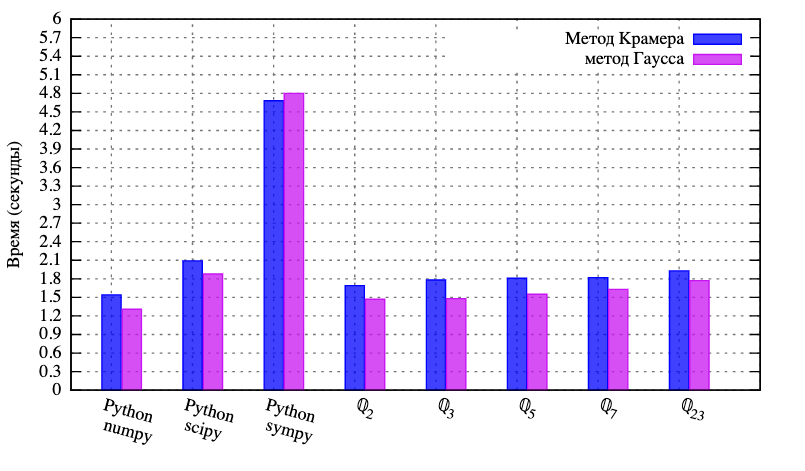
\includegraphics[width=0.85\linewidth]{../gnuplot/single/system/plot.png}}
\caption{Сравнение производительности однопоточных методов для решения СЛАУ.}
\label{img:single:system:1}
\end{figure}

\begin{figure}[H]
\centerline{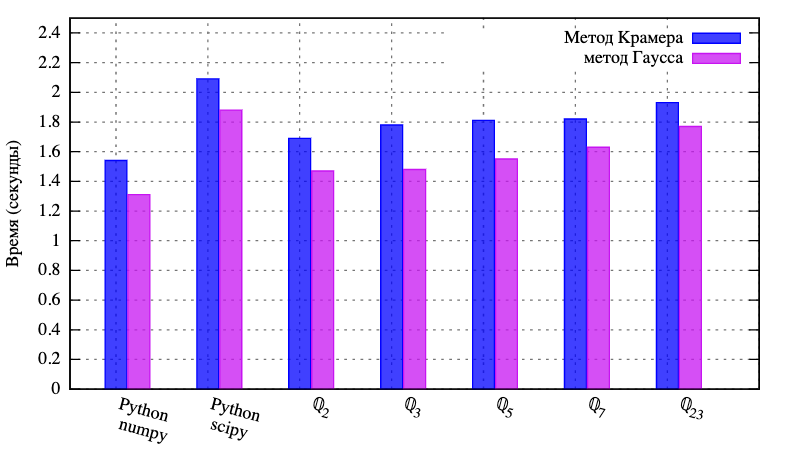
\includegraphics[width=0.85\linewidth]{../gnuplot/single/system/wosymb.png}}
\caption{Сравнение производительности однопоточных методов для решения СЛАУ (без символьного метода).}
\label{img:single:system:2}
\end{figure}

Полученные результаты производительности сопоставимы с результатами, полученными для вычисления определителя матрицы и так же, как и там, методы из пакета |numpy| работают немного быстрее $p$-адических методов, а методы из пакета |sympy| немного дольше. Кроме того, видно, что метод Гаусса работает быстрее, и это является очевидным фактом, так как его алгоритмическая сложность ниже, чем у метода Крамера.

\subsection{Нахождение собственных значений и векторов матрицы}

Для создания многопоточного алгоритма для нахождения собственных значений и собственных векторов матрицы была изучена литература \cite{bib:number:theory, bib:algebra:1, bib:number:borevich}. Результаты работы алгоритма приведены на графике \ref{img:multi:jacoby}.

\begin{figure}[H]
\centerline{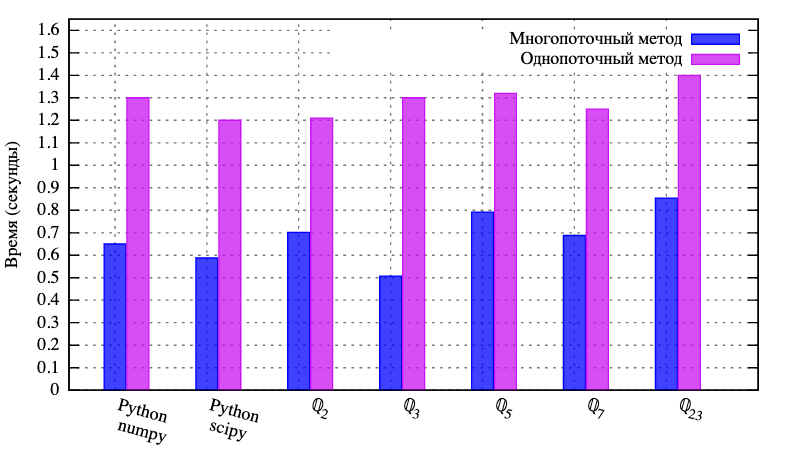
\includegraphics[width=0.85\linewidth]{../gnuplot/multi/jacoby/plot.png}}
\caption{Сравнение методов для нахождения собственных чисел и собственных векторов матрицы.}
\label{img:multi:jacoby}
\end{figure}

Из представленной диаграммы \ref{img:multi:jacoby} видно, что, как и в случае с нахождением решения СЛАУ, многопоточные $p$-адические методы нахождения собственных чисел и векторов не уступают, а в некоторых случаях являются более быстрыми по сравнению с методами из стандартных библиотек ЯП Python. Также видно, что разная база для $p$-адических чисел дает немного различный результат и оптимальной базой является $p=2$ или $p=3$.


\subsection{Решение ОДУ}
Для сравнения времени решения обыкновенных дифференциальных уравнений возьмем простейшее дифференциальное уравнение падающей \mbox{сферы:}

\begin{equation}
\begin{aligned}
\dfrac{\partial z}{ \partial t} = v, \\
\dfrac{\partial v}{ \partial t} = g - \alpha v^2, \\
\alpha = \frac{3\rho_f}{4\rho_k d}C_d.
\end{aligned}
\end{equation}

\noindent Аналитическое решение данного уравнения при $z(0)=0$ и $v(0)=0$ представляет собой следующие функции:

\begin{equation}
\begin{aligned}
z(t)=\frac{\log{(\cosh{(\sqrt{\alpha g} \cdot t})})}{\alpha}, \\
v(t)=\sqrt{\frac{g}{\alpha}} \cdot \tanh{(\sqrt{\alpha g} \cdot t)}.
\end{aligned}
\end{equation}

\noindent Конечная скорость $v_t$ находится из уравнения $\frac{\partial v}{ \partial t}$ и равна $v_t=\sqrt{\frac{g}{\alpha}}$.

В качестве физических параметров для эксперимента будем использовать параметры стандартного мяча для гольфа:

\begin{threeparttable}
\begin{longtable}[H]{lp{0.7\linewidth}}
{$d$} -- диаметр шара & 41 [мм] \\
{$\rho_k$} -- плотность сферы & 1275 [кг/м\textsuperscript{3}] \\
{$\rho_f$} -- плотность жидкости & 1.22 [кг/м\textsuperscript{3}] \\
{$C_d$} -- коэффициент трения & 0.4
\end{longtable}
\end{threeparttable}


При этих параметрах $\alpha$=$7 \cdot 10^{-3}$, а конечная скорость становится равной $v_t=\sqrt{\frac{g}{\alpha}}=37.44$.

Для сравнения методов будем использовать стандартную схему метода Рунге-Кутты 4-го порядка

\begin{equation}%\label{eq:task:2}
\begin{aligned}
k_1 = f(x_n, y_n), \\
k_2 = f(x_n+\frac{h}{2}, y_n+\frac{h}{2}k_1), \\
k_3 = f(x_n+\frac{h}{2}, y_n+\frac{h}{2}k_2), \\
k_4 = f(x_n+h, y_n+hk_3), \\
y_{n+1}=y_n+\frac{h}{6}(k_1+2k_2+2k3+k_4)
\end{aligned}
\end{equation}


\noindent и схему метода Эйлера

\begin{equation}%\label{eq:task:2}
\begin{aligned}
y_{n+1}=y_n+h \cdot f(x_n, y_n).
\end{aligned}
\end{equation}


Разные запуски реализаций решения на ПК дают несколько разное время, поскольку операционная система периодически отбирает ресурсы от запущенной программы для своих нужд. Из нескольких запусков будем записывать минимальное время. Запускать тесты будем $100$ раз. Из нескольких запусков будем записывать минимальное время.

Для наглядности будем сравнивать время нахождения решения ОДУ между классическими методами из таких стандартных библиотек ЯП Python, как |numpy| и |scipy|, и $p$-адическими методами, которые используют числа из $\mathbb{Q}_2$, $\mathbb{Q}_3$, $\mathbb{Q}_5, \mathbb{Q}_5$ и $\mathbb{Q}_{23}$.

\begin{figure}[H]
\centerline{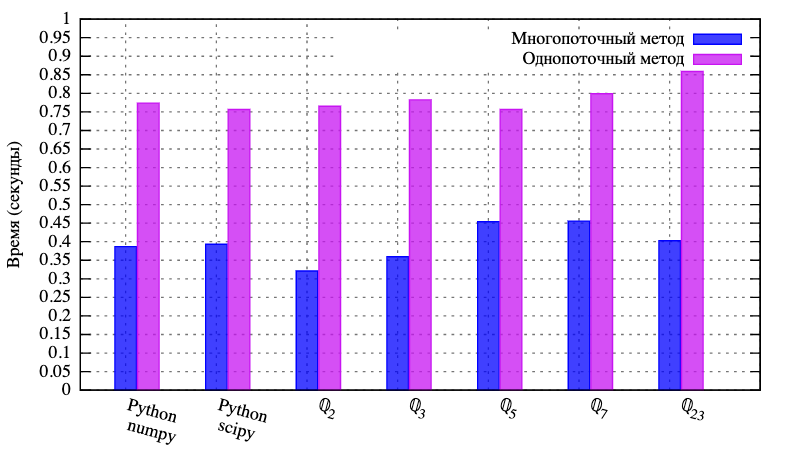
\includegraphics[width=0.85\linewidth]{../gnuplot/multi/euler/plot.png}}
\caption{Сравнение методов для нахождения численного решения ОДУ с помощью метода Эйлера.}
\label{img:multi:ode:euler}
\end{figure}


Как видно из представленной диаграммы \ref{img:multi:ode:euler}, метод Эйлера дает неплохие результаты с использованием параллельной $p$-адической арифметики.


\begin{figure}[H]
\centerline{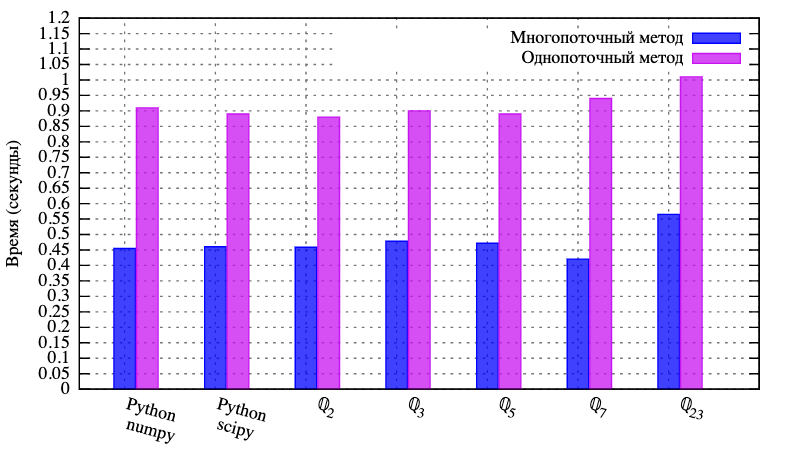
\includegraphics[width=0.85\linewidth]{../gnuplot/multi/rk/plot.png}}
\caption{Сравнение методов для нахождения решения ОДУ с помощью метода Рунге-Кутты 4-го порядка.}
\label{img:comp:ode:rk}
\end{figure}

\begin{figure}[H]
\centerline{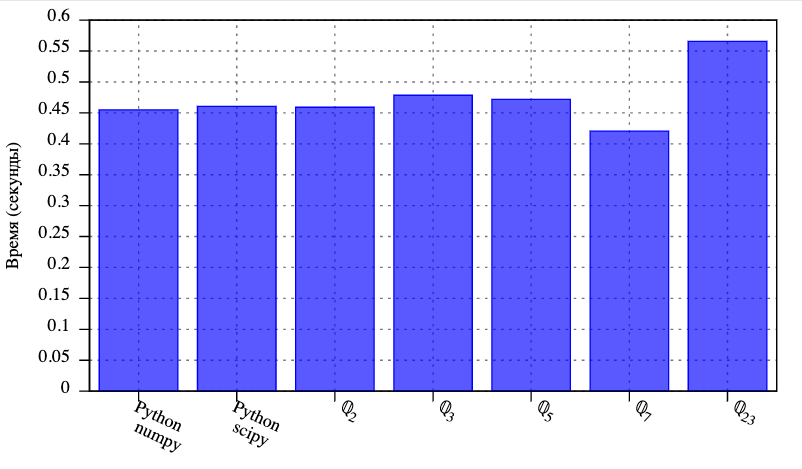
\includegraphics[width=0.85\linewidth]{../gnuplot/multi/rk/multi.png}}
\caption{Сравнение классических методов для нахождения решения ОДУ с помощью метода Рунге-Кутты 4-го порядка и методов с использованием параллельной $p$-адической арифметики.}
\label{img:comp:ode:rk:multi}
\end{figure}

Как видно из представленных диаграмм \ref{img:comp:ode:rk}, \ref{img:comp:ode:rk:multi}, метод Рунге-Кутты 4-го порядка с помощью использования $p$-адической арифметики работает даже лучше, чем классические методы, представленные в стандартных библиотеках, в случае использования многопоточных методов. В случае использования однопоточного метода $p$-адический метод дает сопоставимое с классическим методом время решения.

\subsection{Вычисление матричной экспоненты}

Для создания многопоточного алгоритма для нахождения матричной экспоненты была изучена литература \cite{bib:numbers:morrison, bib:numbers:dixon, bib:ode:3, bib:numbers:limongelli, bib:numbers:mignotte}.

Сравнение вычисления $e^{At}$ производились с использованием использовать 4 параллельных потоков. Параллелизация в данном случае использовалась для одновременного вычисления произведения $\alpha_{j}(t)A^j$.

Для тестов были сгенерированы случайные матрицы размера от \mbox{$100 \times 100$} до \mbox{$500 \times 500$}. Числитель $a$ и знаменатель $b$ каждого рационального элемента $\frac{a}{b}$ сгенерированной матрицы удовлетворяет условию $\abs{a,b} \leq 30$.


\begin{figure}[H]
\centerline{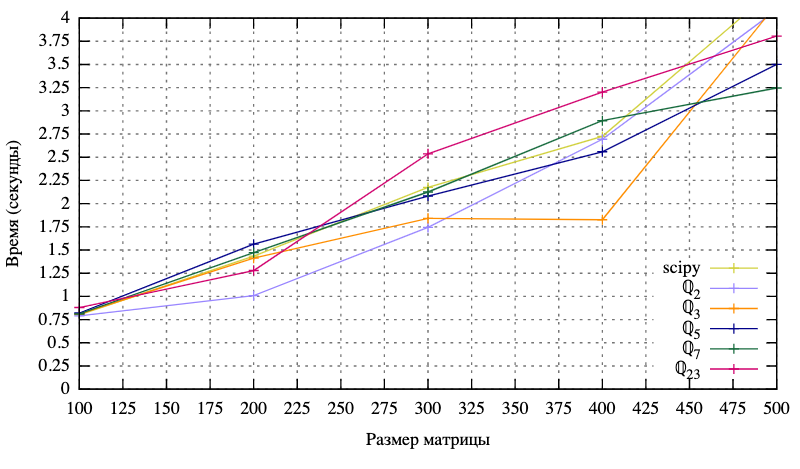
\includegraphics[width=0.85\linewidth]{../gnuplot/exp/plot.png}}
\caption{Сравнение классических и $p$-адических методов для вычисления матричной экспоненты.}
\label{img:exp:plot}
\end{figure}

Как видно из представленного графика \ref{img:exp:plot}, вычисление матричной экспоненты с помощью $p$-адических методов при использовании чисел из $\mathbb{Q}_2, \mathbb{Q}_3, \mathbb{Q}_5, \mathbb{Q}_7$ даёт лучшие результаты, чем аналогичные классические методы из математического пакета |scipy| для ЯП Python.

\conclusion
В течение семестра была разработана многопоточная библиотека для работы с $p$-адической арифметикой, позволяющая применять $p$-адическую арифметику к популярным задачам математики и физики, как это было сделано в приведенных примерах. Помимо этого, на студенческой научной конференции, которая проходила в апреле, был представлен доклад на тему применения $p$-адической арифметики к вычислению матричной экспоненты.

В дальнейшем планируется описать все теоретические и практические аспекты применения $p$-адической арифметики к вычислениям производимым на компьютере, на примере разработанной библиотеки, и закончить оформление библиотеки в виде полноценного пакета для ЯП Python. Кроме того, планируется проведение более подробного тестирования для того, чтобы привести полученные результаты в магистерской выпускной квалификационной работе.

\bibliographystyle{biblio/ugost}
\bibliography{biblio/biblio}


\appendix

\section{Исходный код библиотеки для работы с $p$-адической арифметикой}

% padic
\lstinputlisting[language=Python, numbers=left, showstringspaces=false, breaklines=true, basicstyle=\small, caption=Класс Padic.]{../python/padic/padic.py}

% matrix
\lstinputlisting[language=Python, numbers=left, showstringspaces=false, breaklines=true, basicstyle=\small, caption=Класс Matrix.]{../python/padic/matrix.py}
% cramer
\lstinputlisting[language=Python, numbers=left, showstringspaces=false, breaklines=true, basicstyle=\small, caption=Метод Крамера]{../python/algo/cramer.py}

% Gauss
\lstinputlisting[language=Python, numbers=left, showstringspaces=false, breaklines=true, basicstyle=\small, caption=Метод Гаусса.]{../python/algo/gauss.py}

% Jacoby
\lstinputlisting[language=Python, numbers=left, showstringspaces=false, breaklines=true, basicstyle=\small, caption=Метод Якоби.]{../python/algo/jacoby.py}

% utils: runner
\lstinputlisting[language=Python, numbers=left, showstringspaces=false, breaklines=true, basicstyle=\small, caption=Менеджер для запуска параллельных процессов.]{../python/utils/runner.py}

\end{document}
